\documentclass[a4paper]{article}
\usepackage[utf8x]{inputenc}
\usepackage[T1,T2A]{fontenc}
\usepackage[russian]{babel}
\usepackage{hyperref}
\usepackage{indentfirst}
\usepackage{listings}
\usepackage{color}
\usepackage{here}
\usepackage{array}
\usepackage{multirow}
\usepackage{graphicx}
\setcounter{tocdepth}{3}

\usepackage{caption}
\renewcommand{\lstlistingname}{Программа} % заголовок листингов кода

\usepackage{listings}
\lstset{ %
extendedchars=\true,
keepspaces=true,
language=bash,					% choose the language of the code
basicstyle=\footnotesize,		% the size of the fonts that are used for the code
numbers=left,					% where to put the line-numbers
numberstyle=\footnotesize,		% the size of the fonts that are used for the line-numbers
stepnumber=1,					% the step between two line-numbers. If it is 1 each line will be numbered
numbersep=5pt,					% how far the line-numbers are from the code
backgroundcolor=\color{white},	% choose the background color. You must add \usepackage{color}
showspaces=false				% show spaces adding particular underscores
showstringspaces=false,			% underline spaces within strings
showtabs=false,					% show tabs within strings adding particular underscores
frame=single,           		% adds a frame around the code
tabsize=2,						% sets default tabsize to 2 spaces
captionpos=b,					% sets the caption-position to bottom
breaklines=true,				% sets automatic line breaking
breakatwhitespace=false,		% sets if automatic breaks should only happen at whitespace
escapeinside={\%*}{*)},			% if you want to add a comment within your code
postbreak=\raisebox{0ex}[0ex][0ex]{\ensuremath{\color{red}\hookrightarrow\space}}
}

\usepackage[left=2cm,right=2cm,
top=2cm,bottom=2cm,bindingoffset=0cm]{geometry}


\begin{document}	% начало документа

\begin{titlepage}	% начало титульной страницы

	\begin{center}		% выравнивание по центру

		\large Санкт-Петербургский Политехнический Университет Петра Великого\\
		\large Институт компьютерных наук и технологий \\
		\large Кафедра компьютерных систем и программных технологий\\[6cm]
		% название института, затем отступ 6см
		
		\huge Программирование\\[0.5cm] % название работы, затем отступ 0,5см
		\large Отчет по курсовой работе\\[0.1cm]
		\large Игра: Сапёр\\[5cm]
	\end{center}


	\begin{flushright} % выравнивание по правому краю
		\begin{minipage}{0.25\textwidth} % врезка в половину ширины текста
			\begin{flushleft} % выровнять её содержимое по левому краю

				\large\textbf{Работу выполнила:}\\
				\large Кузовкина Е.О.\\
				\large {Группа:} 23501/4\\
				
				\large \textbf{Преподаватель:}\\
				\large Вылегжанина К.Д.

			\end{flushleft}
		\end{minipage}
	\end{flushright}
	
	\vfill % заполнить всё доступное ниже пространство

	\begin{center}
	\large Санкт-Петербург\\
	\large \the\year % вывести дату
	\end{center} % закончить выравнивание по центру

\thispagestyle{empty} % не нумеровать страницу
\end{titlepage} % конец титульной страницы

\vfill % заполнить всё доступное ниже пространство


% Содержание
\tableofcontents
\newpage

\section{Игровое приложение: Сапёр}

«Сапёр» — компьютерная игра-головоломка.\\

Принцип игры:\\

Плоское или объёмное игровое поле разделено на смежные ячейки (квадраты, шестиугольники, кубы и т. п.), некоторые из которых «заминированы»; количество «заминированных» ячеек известно. Целью игры является открытие всех ячеек, не содержащих мины.\\

Игрок открывает ячейки, стараясь не открыть ячейку с миной. Открыв ячейку с миной, он проигрывает. Мины расставляются после первого хода, поэтому проиграть на первом же ходу невозможно. Если под открытой ячейкой мины нет, то в ней появляется число, показывающее, сколько ячеек, соседствующих с только что открытой, «заминировано» (в каждом варианте игры соседство определяется по-своему); используя эти числа, игрок пытается рассчитать расположение мин, однако иногда даже в середине и в конце игры некоторые ячейки всё же приходится открывать наугад. Если под соседними ячейками тоже нет мин, то открывается некоторая «не заминированная» область до ячеек, в которых есть цифры. «Заминированные» ячейки игрок может пометить, чтобы случайно не открыть их. Открыв все «не заминированные» ячейки, игрок выигрывает.

\subsection{Концепция игрового приложения Сапёр}

Программа представляет собой головоломку, которая позволяет нажимать на ячейки поля, открывая их или обозначая флажком, если игрок считает, что там находится бомба, или вопросительным знаком, если игрок предполагает, что эти ячейки не стоит открывать и там может быть бомба.\\

Приложение отрисовывает игровое поле, на котором располагаются бомбы. Пользователь не видит их. Пользователь может открывать любые ячейки и обновлять игру в любой момент, нажав на смайлик. Игра считается законченой, если пользователь разминировал все бомбы, то есть правильно расставил флажки.

\subsection{Задание}

Разработать приложение под операционные системы Windows 7+ и Android, позволяющее разгадывать головоломку Сапёр. 

\subsection{Минимально работоспособный продукт}

Приложение, которое предоставляет возможность открывать ячейки и ставить флажки.

\subsection{Вывод}

Пояснён выбор темы курсового проекта. Описана концепция игрового приложения Сапёр. Определено задание.

%#######################################################################################################

\section{Проектирование игрового приложения Сапёр}

\subsection{Архитектура приложения}

Был использован шаблон проектирования Model-View-Presenter\\

Его использование обусловленно тем, что:

\begin{enumerate}  
\item[•]  требовалось обеспечить расширяемость приложения, так как существовала некоторая неопределённость по поводу того, какую функциональность должно предоставлять приложение, так как планировалось учесть новые пожелания пользователей
\item[•]  требовалось обеспечить скорость разработки
\item[•]  этот шаблон интересен с учебной точки зрения
\end{enumerate}

Архитектура Модели выглядит следующим образом:
\begin{figure}[H]
	\begin{center}
		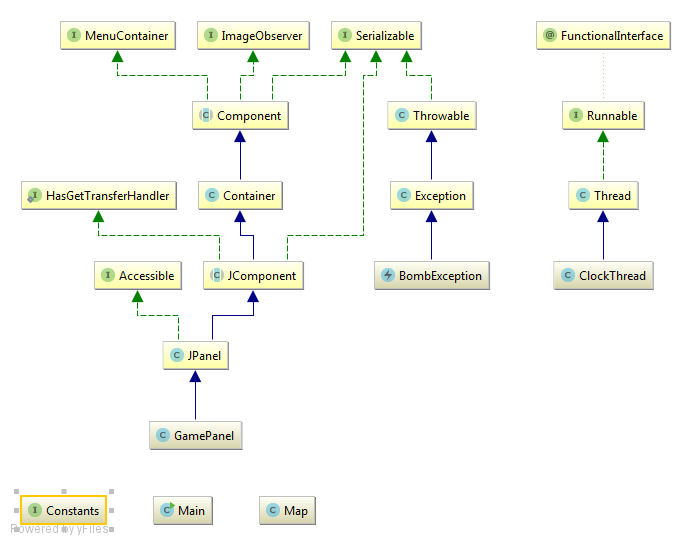
\includegraphics[scale=0.7]{images/diagram0.png}
		\caption{Диаграма классов Модели} 
		\label{pic:pic_name} % название для ссылок внутри кода
	\end{center}
\end{figure}

Модель предоставляет следующую функциональность:

\begin{enumerate}  
\item[•]  Показать длительность игры
\item[•]  Открыть ячейку
\item[•]  Пометить ячейку вопросительным знаком
\item[•]  Показать окончание игры, открытие всех ячеек
\item[•]  Пометить ячейку флажком
\item[•]  Установить игровое поле
\item[•]  Получить ячейки поля
\item[•]  Получить информацию о соседних ячейках
\item[•]  Начать игру заново
\end{enumerate}

\subsection{Диаграмма компонентов}

\begin{figure}[H]
	\begin{center}
		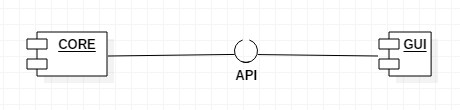
\includegraphics[scale=0.7]{images/diagram1.jpg}
		\caption{Диаграмма компонентов} 
		\label{pic:pic_name} % название для ссылок внутри кода
	\end{center}
\end{figure}

\begin{enumerate}
\item[•] Core -- содержит логическую часть игры, предоставляет данные для пользовательского интерфейса.
\item[•] GUI -- отвечает за взаимодействие с пользователем путём отрисовки изображения на экране и фиксирования команд и событий, которые впоследствии перенаправляет API.
\item[•] API -- управляет Core и API. Указывает GUI, что нужно отрисовывать в данный момент, принимает его оповещания о командах и сигнлах, реагирует на них и, если это необоходимо, связывается с Core для получения данных. 
\end{enumerate}

\subsection{Формат задания игры}

Так как в игре 1 уровень, то пользователь может лишь обновлять поле для старта новой игры и он не может задавать размеры поля и количество мин. Для игры выбрано стандартное поле. 

\subsection{Вывод}

Было решено использовать шаблон проектирования Observer и анти-паттерн Magic Numbers. Была описана функциональность предоставляемая Моделью. Был объяснён формат приложения.

\section{Реализация игрового приложения Сапёр}

\subsection{Используемые версии}

\begin{enumerate}
\item[•]  IntelliJ IDEA 2016.3.1\\
Build IU-163.9166.29\\
For educational use only.\\
JRE: 1.8.0 102-b14 amd64\\
JVM: Java HotSpot(TM) 64-Bit Server VM by Oracle Corporation\\
\item[•]  Java language level: 6
\item[•]  Операционная система: Windows 7 x64
\item[•]  Система автоматической сборки: Gradle 2.14
\end{enumerate}

\subsection{Библиотека Swing}

В данном проекте было принято решение использовать библиотеку Swing.

Swing — библиотека для создания графического интерфейса для программ на языке Java. Он содержит ряд графических компонентов (Swing widgets), таких как кнопки, поля ввода, таблицы и т. д.

\subsection{Процесс разработки игрового приложения}

Было проведено первичное знакомство со Swing и создано приложение, в котором почти не участвует Модель. После получения опыта работы со Swing и принятия решения, что этот фреймворк подходит для решаемой задачи было решено заняться непосредственно развитием функциональности Модели. В итоге выбраный путь позволил корректировать Модель во время разработки таким образом, чтобы с ней было удобно работать.\\

На следующих изображениях поэтапно приведён процесс разработки приложения:

\begin{figure}[H]
	\begin{center}
		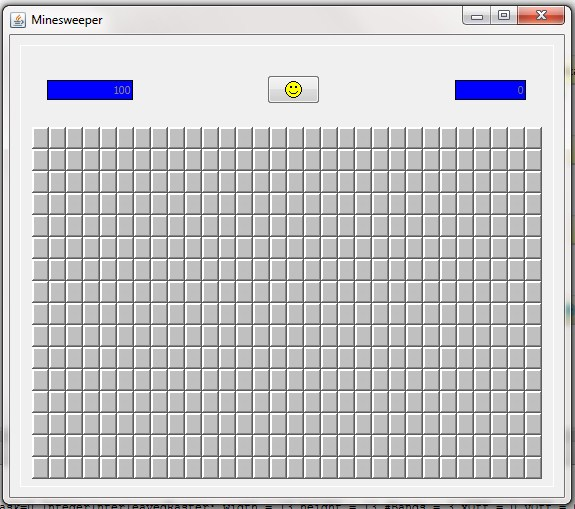
\includegraphics[scale=0.7]{images/1.jpg}
		\caption{Снимок экрана иллюстрирующий игровое окно, до начала игры} 
		\label{pic:pic_name} % название для ссылок внутри кода
	\end{center}
\end{figure}

На рисунке 3 изображён экран, на котором отрисовано закрытое поле, два синих окна, в левом окошке - количество мин, которое необходимо обезвредить, в правом - время от начала игры в секундах. Время не начинает идти пока пользователь не нажмет на ячейку поля.

\begin{figure}[H]
	\begin{center}
		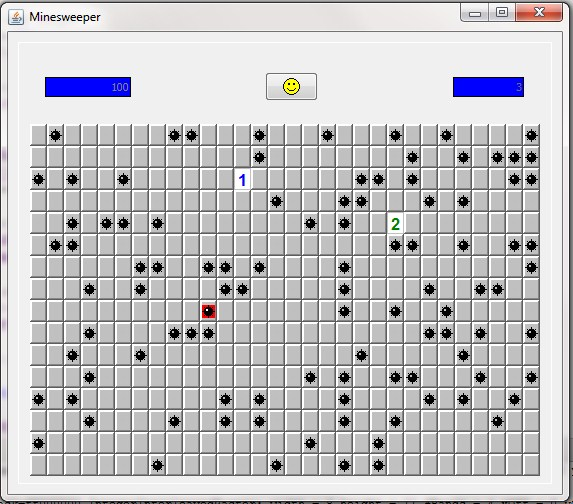
\includegraphics[scale=0.7]{images/2.jpg}
		\caption{Снимок экрана иллюстрирующий вид пользовательского интерфейса после попадания на мину} 
		\label{pic:pic_name} % название для ссылок внутри кода
	\end{center}
\end{figure}

На рисунке 4 пользователь сделал три шага, на третьем шаге он открыл ячейку с миной и взорвался на ней, при этом мина, которая взорвалась обозначается красным, в отличие от остальных. Так как пользователь попал на мину, то окрывается всё поле и игра заканчивается. Для продолжения игры необходимо нажать на смайлик, тогда поле снова становится закрытым и выглядит как на рис. 3.\\

Для открытия ячеек поля пользователь использует левую клавишу мыши и один щелчок.

\begin{figure}[H]
	\begin{center}
		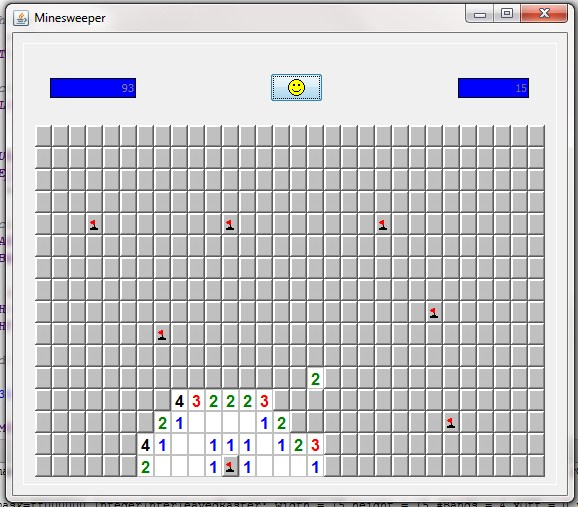
\includegraphics[scale=0.7]{images/3.jpg}
		\caption{Снимок экрана иллюстрирующий расстановку флажков и открытие ячеек} 
		\label{pic:pic_name} % название для ссылок внутри кода
	\end{center}
\end{figure}

На рисунке 5 пользователь открыл несколько ячеек и расставил флажки. Поле с цифрами подсказывает игроку, где находятся мины, то есть где нужно поставить флажок для обезвреживания мины.\\

Для обозначения ячейки флажком, пользователь использует правую клавишу мыши и 1 щелчок. При этом ячейка остается закрытой, то есть неизвестно стоит ли под флажком мина или нет. Для отмены необходимо 2 раза нажать на ячейку, которую необходимо очистить.

\begin{figure}[H]
	\begin{center}
		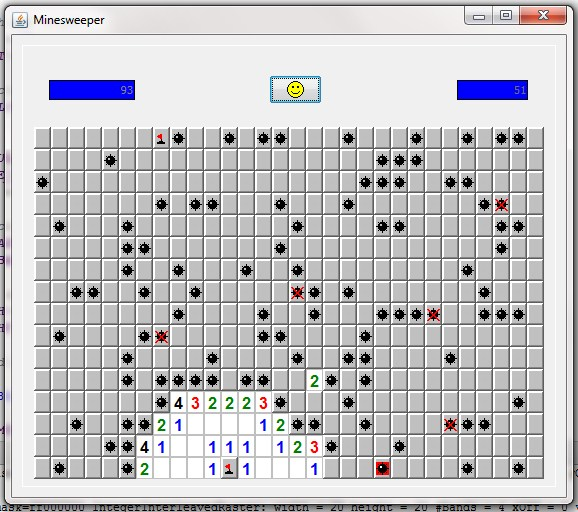
\includegraphics[scale=0.7]{images/4.jpg}
		\caption{Снимок экрана иллюстрирующий обезвреживание нескольких мин} 
		\label{pic:pic_name} % название для ссылок внутри кода
	\end{center}
\end{figure}

На рисунке 6 пользователь попал на мину при открытии следующих ячеек. Те мины, которые были помечены флажком, показаны обезвреженными (зачеркнуты).

\begin{figure}[H]
	\begin{center}
		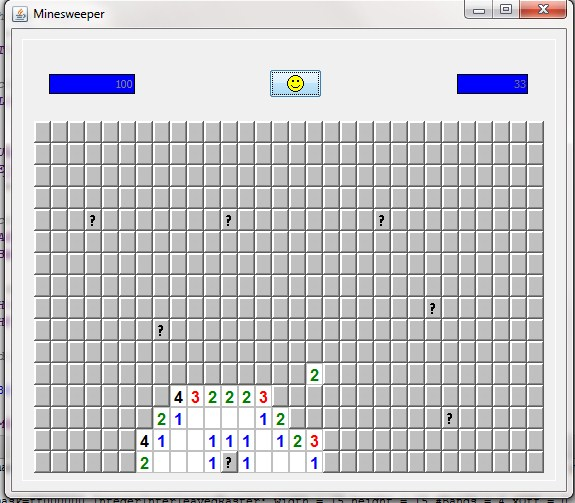
\includegraphics[scale=0.7]{images/5.jpg}
		\caption{Снимок экрана иллюстрирующий расстановку вопросительных знаков} 
		\label{pic:pic_name} % название для ссылок внутри кода
	\end{center}
\end{figure}

На рисунке 7 пользователь расставил вопросительные знаки и открыл несколько ячеек. Вопросительный знак не обезвреживает мины, он лишь помогает пользователю, который сомневается, есть ли в данном месте мина.\\

Для обозначения ячейки вопросительным знаком, пользователь использует правую клавишу мыши и 2 щелчка. При этом ячейка остается закрытой. Для отмены необходимо еще 1 раз нажать на ячейку, с которой необходмо снять вопросительный знак.

\begin{figure}[H]
	\begin{center}
		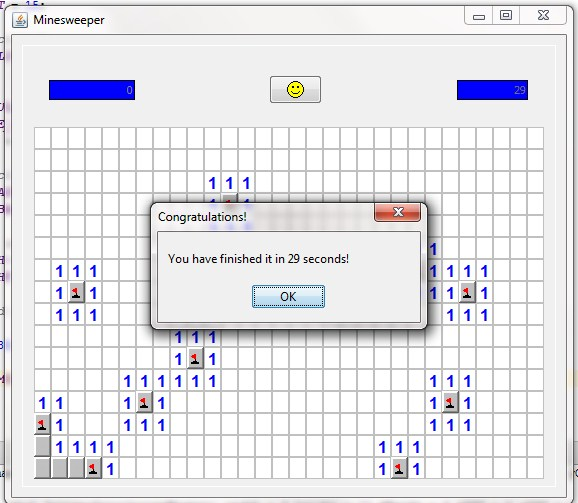
\includegraphics[scale=0.7]{images/6.jpg}
		\caption{Снимок экрана иллюстрирующий оконочание игры} 
		\label{pic:pic_name} % название для ссылок внутри кода
	\end{center}
\end{figure}

На рисунке 8 пользователь правильно разгадал головоломку и появился экран окончания игры с подсчитанным игровым временем (временем, затраченным на разгадку).

\begin{figure}[H]
	\begin{center}
		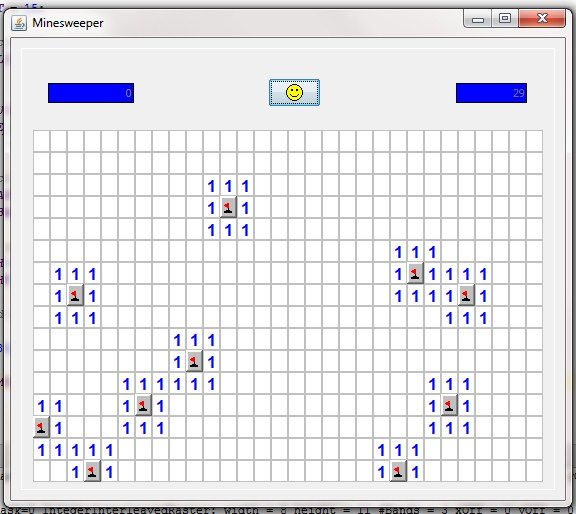
\includegraphics[scale=0.7]{images/7.jpg}
		\caption{Снимок экрана иллюстрирующий полностью открытое поле} 
		\label{pic:pic_name} % название для ссылок внутри кода
	\end{center}
\end{figure}

На рисунке 9 пользователь закрыл окно, которое было на рис. 8 с поздравлениями с успешным прохождением головоломки и подсчитанным временем. После этого всё игровое поле открылось.

\begin{figure}[H]
	\begin{center}
		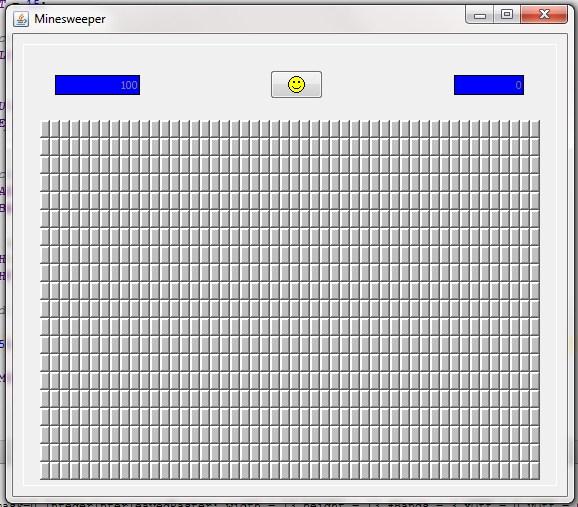
\includegraphics[scale=0.7]{images/8.jpg}
		\caption{Снимок экрана иллюстрирующий увеличенное игровое поле} 
		\label{pic:pic_name} % название для ссылок внутри кода
	\end{center}
\end{figure}

На рисунке 10 показано увеличенное игровое поле. 

\begin{figure}[H]
	\begin{center}
		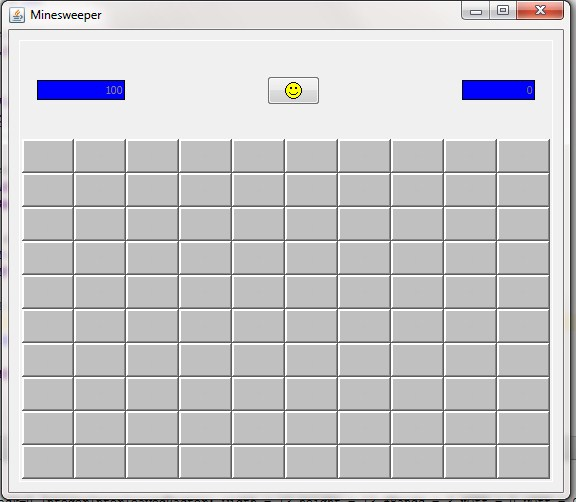
\includegraphics[scale=0.7]{images/9.jpg}
		\caption{Снимок экрана иллюстрирующий уменьшенное игровое поле} 
		\label{pic:pic_name} % название для ссылок внутри кода
	\end{center}
\end{figure}

На рисунке 11 показано уменьшенное игровое поле.\\

В ходе разработки игры для удобства тестирования можно было изменять размеры поля и количество мин. Для окончательной игры было выбрано стандартное значение размеров поля и количество мин для удобства всех пользователей (и новичков, и любителей).

\subsection{Перспективы развития приложения}

Планируется реализовать следующую функциональность:
\begin{enumerate}
\item[•]  добавить изменение размеров поля (пользователем)
\item[•]  добавить изменение количества мин (пользователем)
\item[•]  добавить окно поражения, появляющееся при взрывании на мине
\item[•]  и т.п.
\end{enumerate}

\subsection{Вывод}

Были описаны используемые средства разработки. Кратко описан фреймворк Swing. Был поэтапно описан процесс разработки приложения и пути дальнейшего развития приложения.

\section{Процесс обеспечения качества и тестирование игрового приложения Сапёр}

Для проверки корректности работы проводилось ручное тестирование.

\subsection{Тестирование}

Тестирование проводилось по следующему сценарию:
\begin{enumerate}
\item[1]  Запустить приложение, проверить отрисовку поля и окошек с количеством мин и игровым временем
\item[2]  Открыть любую ячейку поля, проверить, что в ней находится, есть ли цифры показывающие, где скорее всего находится мина
\item[3]  Если попалась мина, то нажать на смайлик и начать игру заново (вернуться в п.2), проверить работает ли обновление игрового поля и старт новой игры
\item[4]  Если открылись ячейки, то рассчитать, где находится мина и поставить на ней флажок, пометить вопросительным знаком все сомнительные ячейки (те, в которых может быть мина, а может и ничего не быть), проверить ставятся ли флажки, вопросительные знаки
\item[5]  Открыть следующие ячейки, в которых скорее всего нет мины
\item[6]  При попадании на мину начать игру заново (вернуться в п.2), проверить открывается ли все игровое поле, чтобы показать расположение всех мин
\item[7]  Продолжить открытие ячеек (как описано в п.4-п.6)
\item[8]  В случае победы проверить правильность информации в окне поздравлений, закрыть его и попробовать начать игру заново, нажав на смайлик
\item[9]  Нажать на кнопку выхода и закрыть приложение
\end{enumerate}

\subsection{Вывод}

Был описан процесс тестирования приложения.

\section{Выводы}

Было разработано игровое приложение Сапёр. Была изучена библиотека Swing и патерн проектирования Model-View-Presenter. Созданое в ходе работы приложение было протестировано, также были определены возможные перспективы развития функциональности приложения. В дальнейшем планируется улучшение приложения, а также исправление возможных недочетов.

\section{Приложение}

Исходный код можно найти в репозитории\footnote{https://github.com/kuzo-liza/Minesweeper} на ресурсе GitHub

\subsection{Листинги}

\lstinputlisting{../src/main/java/minesweeper/logic/Map.java}
\lstinputlisting{../src/main/java/minesweeper/logic/BombException.java}

\lstinputlisting{../src/main/java/minesweeper/gui/Main.java}
\lstinputlisting{../src/main/java/minesweeper/gui/GamePanel.java}
\lstinputlisting{../src/main/java/minesweeper/gui/ClockThread.java}

\lstinputlisting{../src/main/java/minesweeper/Constants.java}
 
\end{document}